\chap{Introducción}{intro}
\graphicspath{{figs/cap2}}

Este capítulo introductorio se divide en tres secciones: 

\begin{itemize}
    \item[-] En la primera sección (\ref{sec:inter}) se presenta la motivación y antecedentes enmarcados en el contexto de esta investigación, definiendo 
    así también el objetivo de la misma.
    \item[-] En la segunda sección (\ref{sec:tfe}) se describen brevemente conceptos generales de teoría fractal e invariantes de escalas, los cuales son
    fundamentales para el desarrollo de este trabajo.
    \item[-] En la tercera sección (\ref{sec:univ}) se presentan y se caracterizan tres de las clases de universalidad más relevantes, conocidas como 
    KPZ (Kardar-Parisi-Zhang), EW (Edwards-Wilkinson) y Poisson.
\end{itemize}

Gran parte de esta introducción estará basada en el libro de 
Barabási, A.L. y Stanley, H.E. (1995), \textit{Fractal concepts in surface growth} \cite{barabasi}. Para mayor detalle en los temas desarrollados en este capítulo
se recomienda la lectura de este libro.

\sect{interfaces fuera del equilibrio en la naturaleza}{inter}

Parafraseando a Barabási y Stanley (1995) \cite{barabasi}, gran parte de nuestras vidas tiene lugar en la superficie/interfaz de algo. En efecto, es probable que usted se 
encuentre sentado sobre una silla en este momento, o más bien, sobre la superficie de la misma. Por otro lado, la humanidad entera vive en la superficie de la Tierra, que 
a su vez constituye una interfaz entre el espacio exterior y el interior de nuestro planeta, vivimos en una interfaz. Si se profundiza en esta idea, es posible 
llegar a pensar que conceptualizamos en función de interfaces. En otro sentido, un sentido más físico, es interesante notar el poder del concepto de interfaz como 
clasificador y descriptor de fenómenos naturales. 

Puede parecer aburrido al principio, dado que observando brevemente a su alrededor encontrará que la mayoría de las cosas que nos rodean son superficies/interfaces que 
parecieran ser estáticas y no presentar variaciones en el tiempo, las cosas que no cambian suelen ser aburridas. Sin embargo, si se observa 
con mayor detalle, quizás en otra escala (temporal o espacial), podremos encontrar una riqueza dinámica muy extensa, asombrosa, y muchas veces universal.

A modo de ejemplo, considere nuevamente la superficie de la Tierra, si se observa desde el espacio, la misma parecería ser una superficie suave y estática,
sin embargo, es claro que no es así. La superficie de la tierra es rugosa vista en la escala espacial correcta y está en constante cambio si la observamos en el 
intervalo de tiempo adecuado.  Dicho de otra manera, la morfología de una interfaz o una estructura puede cambiar al observarla en diferentes escalas. 

Por otro lado, es posible encontrar también ejemplos en la naturaleza en los que la morfología de una interfaz o estructura no cambia al observarla en diferentes 
escalas. En este caso, la interfaz o estructura es \textit{auto-similar} o \textit{fractal}. Más aún, existen ejemplos en los que la morfología no cambia, pero solo si 
el cambio de escala es distinto en diferentes direcciones. En este caso, se dice que el objeto tiene la propiedad de ser \textit{auto-afín}. Precisaremos estos conceptos en 
la sección siguiente. 

De momento vamos a conformarnos con observar que la naturaleza es rica en estructuras y fenómenos que pueden ser descritos en términos de interfaces fuera del equilibrio. 
Algunos ejemplos de ello, muy diferentes microscópicamente, son los que siguen.

\textbf{Propagación de frentes de incendio:} Este es un fenómeno muy habitual en la naturaleza, es posible observarlo sobre una hoja de papel o bien, tristemente, 
    en un bosque. En ambos casos es fácil distinguir una interfaz entre el papel o el bosque quemado y el resto, dando lugar al conocido frente de incendio. Este es un 
    ejemplo de una interfaz que se desplaza sobre un medio desordenado, tanto el papel como el bosque presentan una estructura irregular y heterogénea. En la figura 
    \ref{fig:incendio} se muestra un el perfil del frente de incendio sobre una hoja de papel quemada. Nótese la forma de la interfaz, en principio de apariencia 
    aleatoria \cite{zhang1992modeling,provatas1995scaling,PhysRevLett.79.1515}.

\textbf{Flujo de fluidos en medios porosos:} Si alguna vez derramó café sobre una hoja de papel, probablemente haya notado que el café fluye por el papel, 
    formando una interfaz entre la parte del papel que está mojada y la que no lo está. Este es otro ejemplo de una interfaz que se desplaza sobre un medio 
    desordenado. Una vez que el café es absorbido por el papel, por el fenómeno de capilaridad, la interfaz se estabiliza dejando una estructura característica que con las herramientas 
    adecuadas puede ser descrita cuantitativamente \cite{Jullien1992SurfaceD,PhysRevLett.110.035501}.

\newpage
\begin{figure}[t]
    \centering
    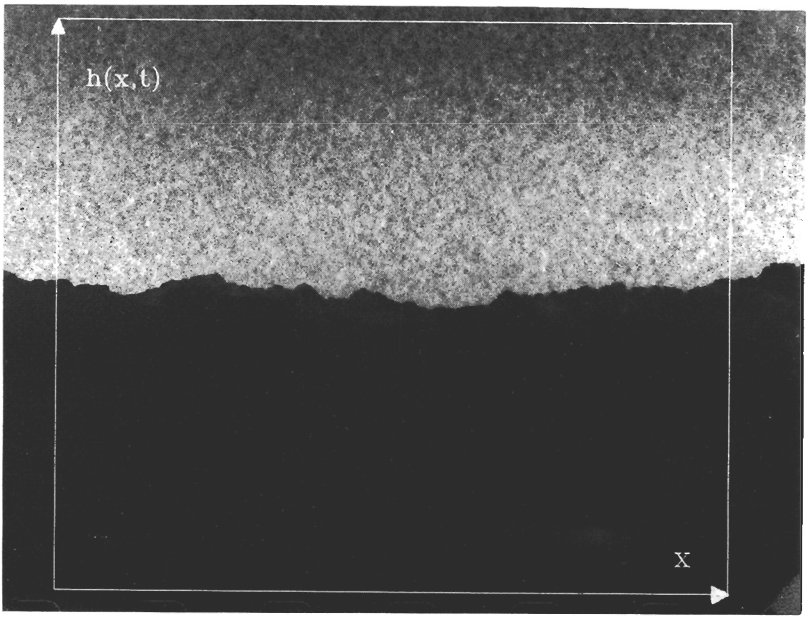
\includegraphics[width=.6\textwidth]{paper_burned.png}
    \caption[Perfil de un frente de incendio sobre una hoja de papel]{Perfil de un frente de incendio sobre una hoja de papel. Figura extraída de Ref. \cite{zhang1992modeling}.}
    \label{fig:incendio}
\end{figure}


\textbf{Mecanismo de defensa de las \textit{abejas gigantes}:} Las \textit{abejas gigantes} (\textit{Apis dorsata}), son una especia de abeja nativa del sudeste asiático, 
Indonesia y Australia. Estas abejas son conocidas por su agresividad y por defender su colmena a toda costa. Uno de sus variados mecanismos de defensa es muy peculiar,
cuando la colmena se ve amenazada por insectos más grandes, como avispas, las abejas, que se encuentran alrededor de la colmena, colectivamente se coordinan para 
producir olas o frentes que espantan a los predadores\footnote{Si se encuentra leyendo esto en una computadora puede mirar un video de este comportamiento 
\href{https://youtu.be/8bNKU8GRYmU}{aquí}.} \cite{kastberger2014speeding,kastberger2013social,kastberger2008social}. En la figura \ref{fig:abeja} se muestra una secuencia de imágenes de este comportamiento, similar a las olas humanas que se dan en los estadios de fútbol \cite{farkas2002mexican,farkas2003human}.

\begin{figure}[!b]
    \centering
    \includegraphics[width=.9\textwidth]{bee_wave.png}
    \caption[Mecanismo de defensa de las \textit{abejas gigantes}.]{Secuencia de imágenes que muestra a las \textit{abejas gigantes} haciendo la ``ola'' como mecanismo de defensa. Figura extraída de Ref. \cite{youtube}.}
    \label{fig:abeja}
\end{figure}
%\newpage

\textbf{Crecimiento de bacterias:} Otro ejemplo de tipo biológico es el crecimiento de colonias de bacterias. En la figura 
\ref{fig:bacteria} se muestra la morfología característica del crecimiento de una especia de bacteria denominada \textit{Bacillus subtilis} sobre un medio de cultivo. 
Se observa que la estructura de la interfaz es sensible a la concentración de nutrientes y otros parámetros experimentales, de modo que la forma de la interfaz tiene 
información sobre el medio de cultivo \cite{matsushita1990diffusion,bhattacharjee2022chemotactic}.


\begin{figure}[ht]
    \centering
    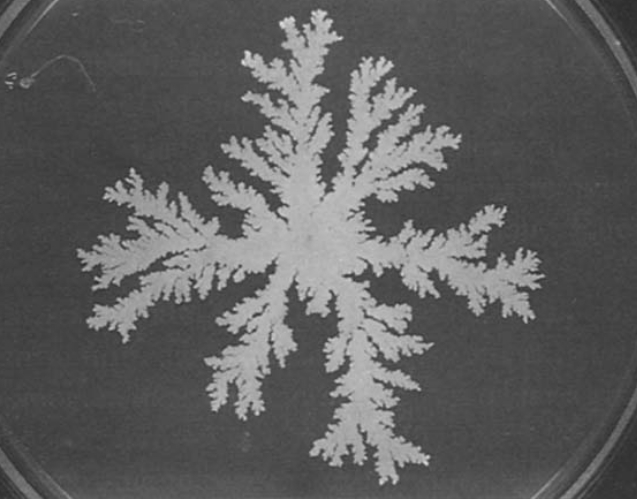
\includegraphics[width=\imsize]{Bacteria.png}
    \caption[Crecimiento de bacterias \textit{Bacillus subtilis}.]{Crecimiento de bacterias \textit{Bacillus subtilis}. Figura extraída de \cite{matsushita1990diffusion}.}
    \label{fig:bacteria}
\end{figure}

\textbf{Frentes de infección:} En epidemiología es posible definir frentes de infección, en donde la interfaz podría entenderse como la frontera 
entre la población infectada y la población no infectada. En el año 1900 la bacteria \textit{Y. pestis} llegó sobre algún pasajero (humano o animal) proveniente de Oriente
al puerto de San Francisco en Estados Unidos. Esta bacteria es la causante de la peste bubónica, una enfermedad mortal que dio lugar a la Peste Negra en Europa 
en el siglo XIV. Los notables avances en la medicina y la higiene desde aquel entonces han reducido el impacto de esta enfermedad. Sin embargo, la bacteria 
sigue presente en el territorio de Estados Unidos, dado que se mantiene endémica sobre la población de roedores, ardillas y conejos. Por esto, se presentan casos 
esporádicos aún en la actualidad. Observando el registro de casos desde 1900 hasta 2012 puede construirse la figura \ref{fig:infeccion}, en al que se ve cómo la peste 
progresa lentamente desde la costa oeste de Estados Unidos hacia la costa este, a unos 50 km por año, trasladada fundamentalmente por los animales pequeños. Esta 
situación constituye una preocupación real dado que no se sabe qué pasara cuando llegue a las grandes ciudades del este de Estados Unidos, donde se encuentra 
la mayor densidad de población, humana y de roedores \cite{mate_sist_bio,barbieri2020soil,stenseth2008plague}.
\newpage

\begin{figure}[ht]
    \centering
    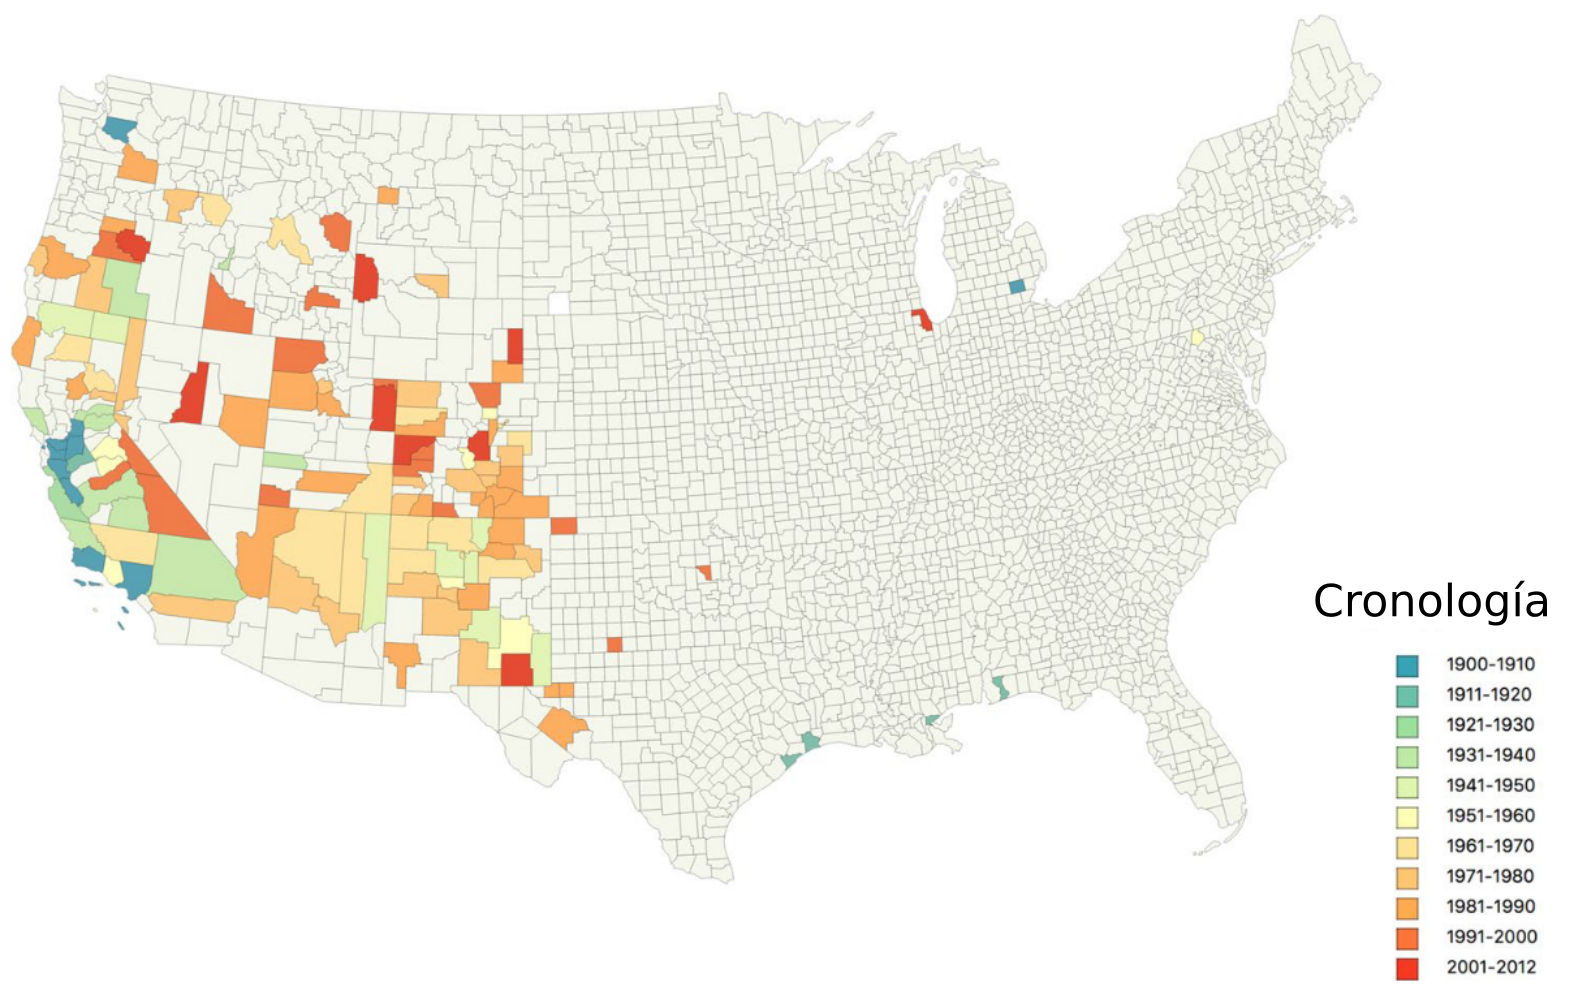
\includegraphics[width=\imsizeL]{peste_eeuu.png}
    \caption[Evolución de la plaga en EE.UU.]{Evolución de la plaga en EE.UU., se muestran coloreados los condados donde se reportó por primera vez un caso y el color indica la cronología. Figura extraída de Ref. \cite{barbieri2020soil}.}
    \label{fig:infeccion}
\end{figure}

\subsection*{Discusión}

En muchos de estos ejemplos notamos que la aleatoriedad, ya sea de la composición del papel que se quema, o bien, del movimiento de las bacterias en el medio de cultivo,
constituye un aspecto crucial en la morfología de las interfaces en cuestión. Por otro lado, observamos que algunos otros casos corresponden con comportamientos o 
dinámicas subyacentes complejas, tal es el caso de las olas de abejas y los frentes infección epidemiológicos. 

Lo interesante es que, sea el fenómeno que sea, la forma de la interfaz tiene información sobre la física subyacente. Más aún, a menudo es posible
encontrar conexiones fundamentales entre problemas esencialmente diferentes. En la sección siguiente presentamos brevemente las herramientas más comúnmente 
utilizadas para estudiar y clasificar las interfaces y sus dinámicas. 

\sect{Conceptos de escala}{tfe}

Para presentar las herramientas y conceptos fundamentales vamos a utilizar como ejemplo ilustrativo un modelo de crecimiento simple y conocido, llamado crecimiento balístico (diremos modelo BD, por \textit{Ballistic Deposition}). La idea es entender las propiedades fundamentales y universales del crecimiento de interfaces, dejando los detalles del proceso de lado.

El proceso del modelo BD es el siguiente: una partícula es liberada en una posición aleatoria, con distribución uniforme, sobre una superficie 
plana a una distancia mayor que la altura máxima de la interfaz. La partícula cae en línea recta hasta entrar en contacto con la superficie, punto en el 
cual se fija. En la figura \ref{fig:bd} se muestra esquemáticamente este proceso. Iterando con $N$ partículas obtenemos el crecimiento balístico. Consideraremos por simplicidad, pero sin pérdida de generalidad, el caso unidimensional.

\begin{figure}[!b]
    \centering
    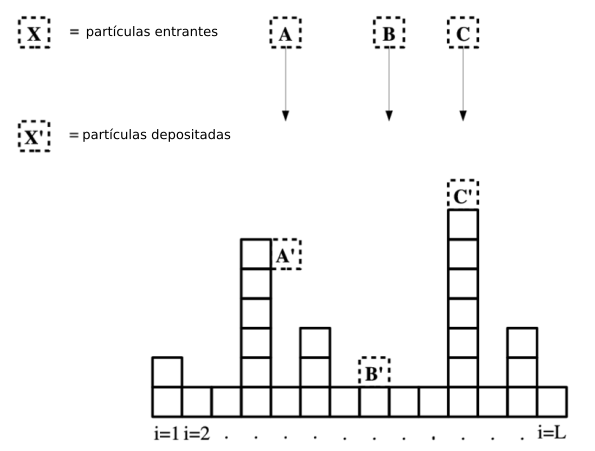
\includegraphics[width=\imsize]{BD.png}
    \caption[Esquema del modelo BD discreto.]{Esquema del modelo BD discreto: la partícula A cae hasta fijarse a la superficie al entrar en contacto de manera lateral con la 
    misma, por su parte las partículas B y C, se fijan a la superficie de manera vertical. La posibilidad de fijación lateral es de gran relevancia en la morfología 
    de la interfaz. Figura extraída de Ref. \cite{farahzadi2008systematic}.}
    \label{fig:bd}
\end{figure}

\ssect{Ancho de la interfaz}{width}

Para comenzar a caracterizar la interfaz primero definimos la altura de la misma como $h(x,t)$, que da la altura en la posición $x$ a tiempo $t$. A partir de esta 
podemos definir también la altura media de la interfaz $h_m(t)$ como,
\begin{equation}
h_{m}(t) = \langle h(x,t) \rangle_x =  \frac{1}{L}\int_{0}^{L}h(x,t)dx,
\end{equation}
donde $L$ es la longitud de la superficie de apoyo, o bien, el tamaño del sistema en la dirección transversal al crecimiento. Si la cantidad de partículas que llegan a una determinada posición por unidad de tiempo es constante, entonces la altura media crece linealmente con el tiempo
\begin{equation}
    h_{m}(t) \propto t.
\end{equation}

Una cantidad esencial para estudiar el crecimiento es el ancho medio de la interfaz, dado simplemente por la desviación estándar de la altura, es decir,
\begin{equation}
\omega(L,t) = \overline{\sqrt{\langle (h(x,t) - h_m(t))^2 \rangle_x}}= \overline{\frac{1}{\sqrt{L}}\left(\int_{0}^{L}(h(x,t) - h_m(t))^2 dx\right)^{1/2}},
\end{equation}
donde $\overline{\cdots}$ significa promedio sobre distintas realizaciones.
Si graficamos el ancho como función del tiempo para el modelo BD, obtenemos la figura \ref{fig:width}, que a su vez es un resultado representativo de lo que 
resulta típicamente al observar esta cantidad.\footnote{Se utilizó $t = n/L$ donde $n$ es el número de iteraciones realizadas del modelo BD.} Vemos que, inicialmente, el ancho crece siguiendo una ley de potencia, 
\begin{equation}
\omega (L,t) \propto t^{\beta},
\end{equation}
donde $\beta$ se conoce como el exponente de crecimiento, el cual caracteriza la dependencia temporal del proceso de rugosidad. Luego de un tiempo de saturación $t_x$, 
el ancho deja de crecer y se mantiene constante en un valor $\omega_{sat}$.

\begin{figure}[!b]
    \centering
    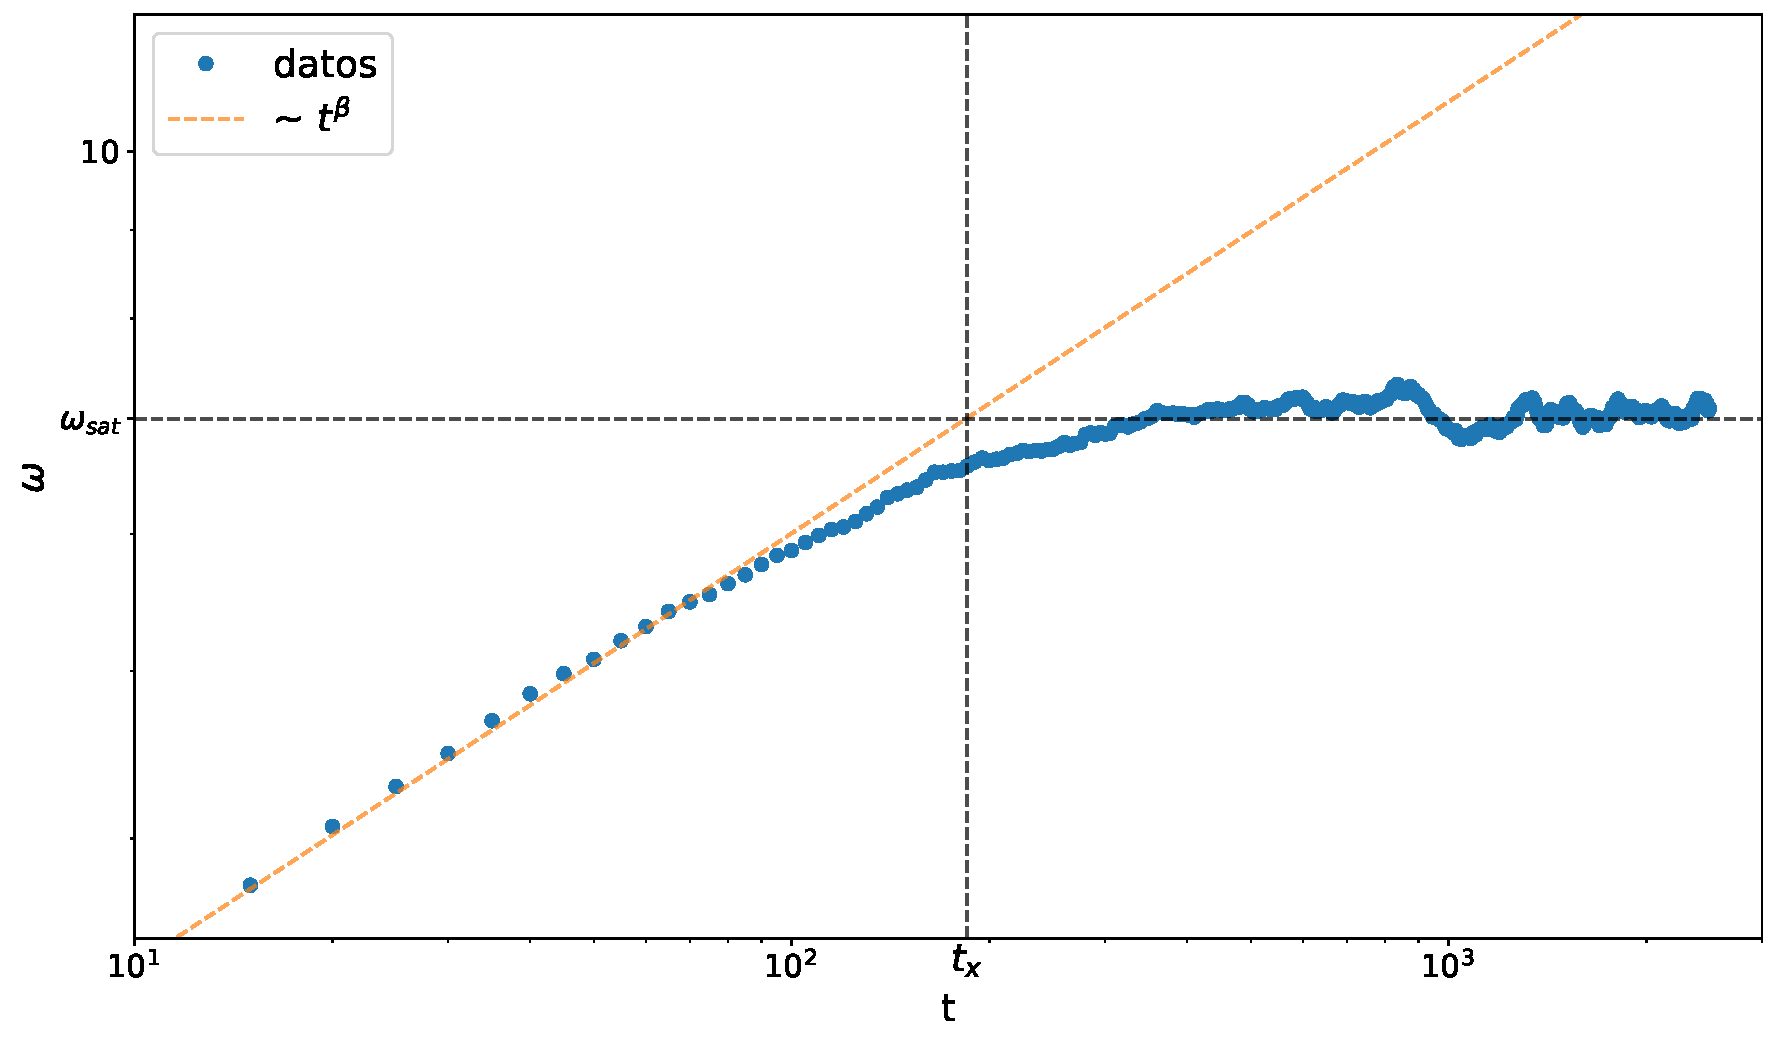
\includegraphics[width=\imsizeL]{width.pdf}
    \caption[Ancho de la interfaz como función del tiempo para el modelo BD discreto.]{Ancho de la interfaz $\omega$ como función del tiempo para el modelo BD discreto con $L = 200$, $N = 50000$ partículas y 500 realizaciones. Se observa el régimen de crecimiento, 
    donde $\omega(L,t \ll t_x) \propto t^\beta$ y el régimen de saturación $\omega(L,t \gg t_x) = \omega_{sat}$, que se alcanza a un tiempo de saturación $t_x$.}
    \label{fig:width}
\end{figure}


Consideremos ahora la figura \ref{fig:width_L} (a), donde se muestra la evolución del ancho para distintos tamaños de sistema $L$. Vemos que, tanto el 
valor de saturación del ancho $w_{sat}$ como $t_x$ crecen con el tamaño del sistema. En particular, puede verse que se cumple
\begin{equation}
\omega(L,t \gg t_x) \propto L^\alpha,
\end{equation}
donde $\alpha$ es el exponente de rugosidad. Mientras que el tiempo de correlación crece como,
\begin{equation}
t_x \propto L^{z},
\end{equation}
donde $z$ es el exponente dinámico.

Teniendo estas leyes de potencia en cuenta, es posible colapsar las curvas de la figura \ref{fig:width_L}a en una única curva (figura \ref{fig:width_L}b), dividiendo $\omega(L,t)$ por $\omega_{sat} \propto L^\alpha$. De esta manera hacemos que todas las curvas saturen en el mismo valor. Luego, para hacer coincidir el tiempo de saturación, escaleamos el tiempo por $t_x \propto L^{z}$. Con este argumento obtenemos la relación de escaleo de \textit{Family-Vicsek} \cite{Family_1985},

\begin{equation}
    \omega(L,t) \propto L^{\alpha} f\left(\frac{t}{L^z}\right),
\end{equation}
donde $f(u)$ es una función universal que cumple,

\begin{equation}
    f(u) =
    \begin{cases}
        u^\beta & \text{si } u \ll 1 \\
        cte & \text{si } u \gg 1.
    \end{cases}
\end{equation}

\begin{figure}[!b]
    \hspace*{-1cm}
    \begin{subfigure}{.55\textwidth}
      \centering
      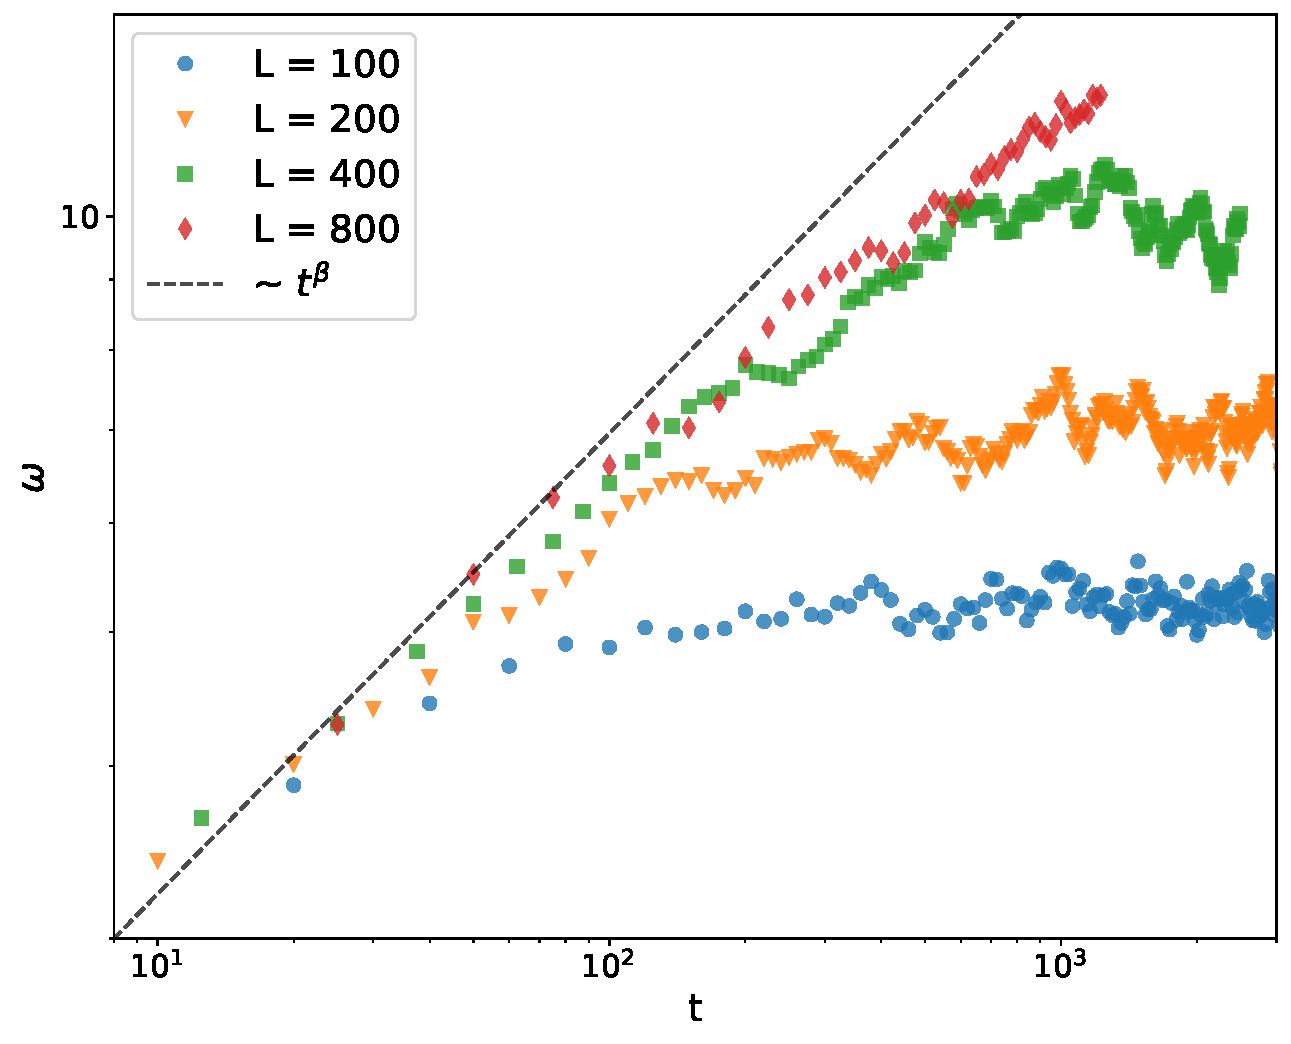
\includegraphics[width=\textwidth]{width_L.pdf}
      \caption{}
    \end{subfigure}
    \begin{subfigure}{.55\textwidth}
      \centering
      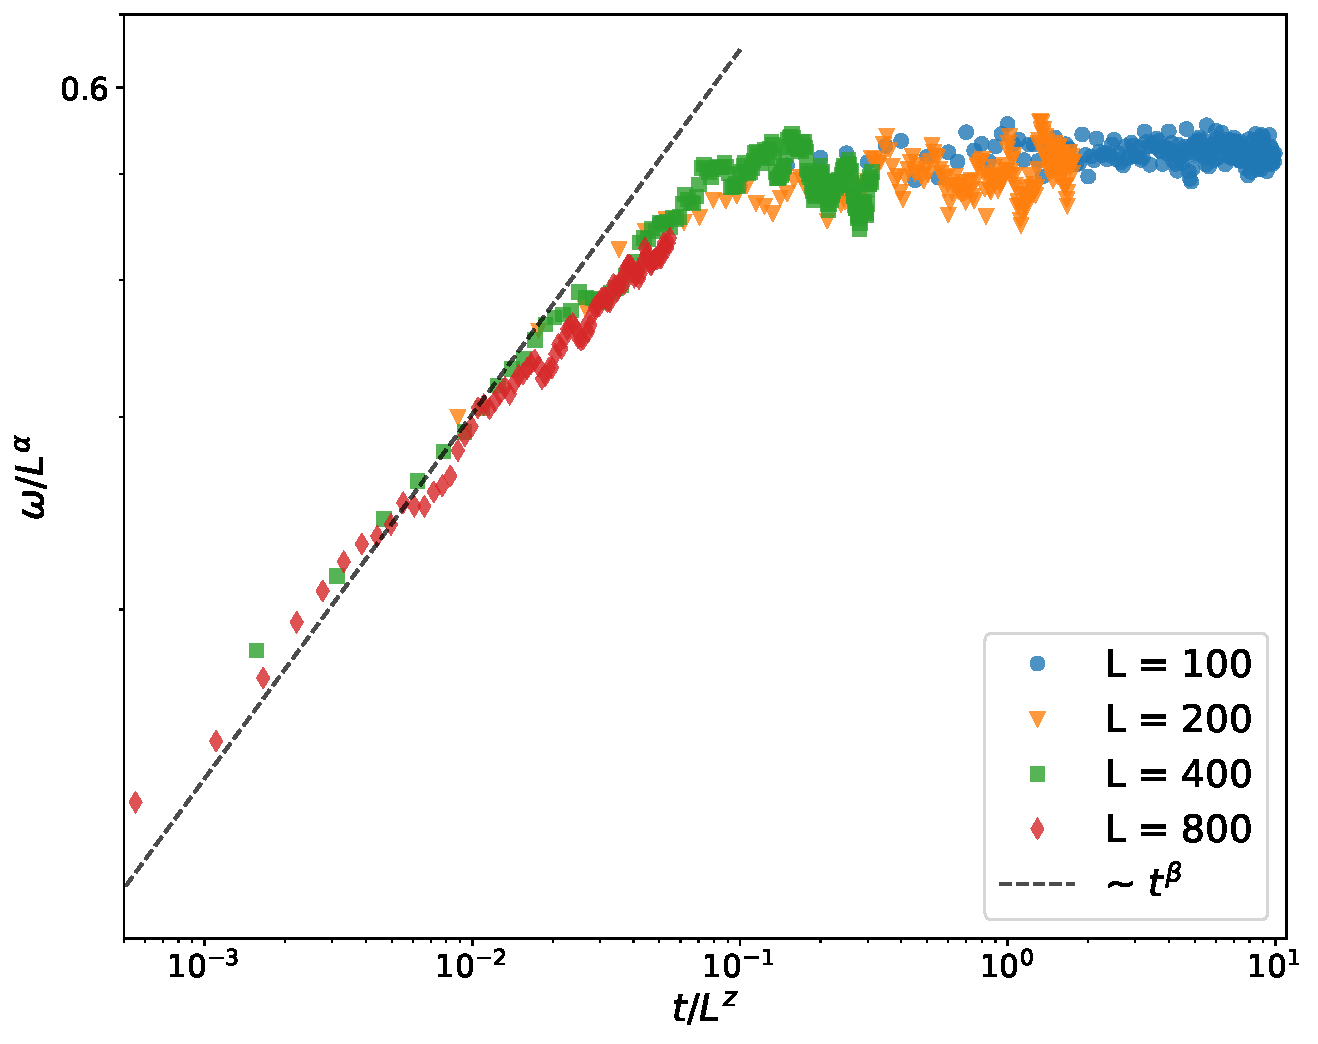
\includegraphics[width=\textwidth]{width_L_colapse.pdf}
      \caption{}
    \end{subfigure}
    \caption[Ancho de la interfaz en el modelo BD discreto para distintos tamaños de sistema y colapso de curvas.]{\textbf{(a)} Ancho de la interfaz como función del tiempo para el modelo BD discreto con distintos tamaños de sistema $L$ y $N = 10^6$ partículas. \textbf{(b)} Colapso de las curvas que permite obtener los exponentes de rugosidad $\alpha$ y dinámico $z$.}
    \label{fig:width_L}
\end{figure}


Hasta el momento hemos presentado tres exponentes que describen cuantitativamente diferentes aspectos del crecimiento de la interfaz, estos son, 
$\beta$, $\alpha$ y $z$. Es importante notar que estos exponentes no son independientes entre sí, consideremos el momento donde el ancho del frente
alcanza su valor de saturación, es decir, $t \approx t_x$. En este momento, el ancho de la interfaz puede expresarse de dos formas equivalentes, 
considerando el régimen de crecimiento $\omega(L,t_x) \propto t_x^\beta$, mientras que en el régimen de saturación $\omega(L,t) \propto L^\alpha$, usando además
que $t_x \propto L^z$, obtenemos que 
\begin{equation}
    z = \frac{\alpha}{\beta}.
\end{equation}

Por otro lado, desde un punto de vista físico, la pregunta que debe hacerse es: ¿por qué el ancho satura en un valor finito? Más aún, ¿por qué el ancho satura en un valor que depende del 
tamaño del sistema? Esto se debe a que el crecimiento de la interfaz está correlacionado. En el caso del modelo BD esto se corresponde con el hecho de que 
las partículas pueden pegarse lateralmente al frente, de modo que la altura en la posición donde cae esa partícula será igual o mayor a la de sus vecinos. Esta correlación 
microscópica se propaga lateralmente sobre la interfaz a medida que pasa el tiempo, de modo que la altura de un punto puede impactar a una distancia cada vez mayor. De 
esta manera comienzan a crearse regiones en la interfaz con una longitud característica $\xi_{||}(t)$ denominada longitud de correlación dinámica. Dado que el sistema es de tamaño 
finito $L$, la longitud de correlación no puede ser mayor que $L$, es decir,
\begin{equation}
    \xi_{||}(t) \propto L \quad \text{con } \quad t \gg t_x.
\end{equation}
Además, dado que $t_x \propto L^z$, en el tiempo de saturación se cumple $\xi_{||} \propto t_x^{1/z}$, que de hecho también vale para $t \ll t_x$,
\begin{equation}
    \xi_{||}(t) \propto t^{1/z}.
\end{equation}
De modo que el ancho de la interfaz deja de crecer cuando la longitud de correlación alcanza el tamaño del sistema, fijando así la máxima magnitud de 
fluctuaciones que puede tener la interfaz. Así mismo, queda claro por qué el valor de saturación depende del tamaño del sistema, al ser más grande el sistema lleva
más tiempo correlacionarlo por completo y por lo tanto el ancho de la interfaz alcanza un valor mayor antes de saturar.

\ssect{Factor de estructura de la interfaz}{sq}

Otro observable de utilidad para caracterizar el crecimiento de interfaces es el factor de estructura $S(q,t)$, definido en términos de $h(x,t)$ como
\begin{equation}
    S(q,t) = \overline{\tilde{h}(q,t)\tilde{h}(-q,t)},
\end{equation} 
donde
\begin{equation}
    \tilde{h}(q,t) = \int h(x,t) e^{-iqx} dx.
\end{equation}
es la transformada de Fourier sobre el espacio del campo de desplazamiento o alturas $h(x,t)$ que definen la interfaz. En este caso, si la condición inicial de la interfaz es plana, el factor de estructura sigue las siguientes leyes de potencia según sea $\xi_{||}(t)$,
\begin{equation}
    S(q,t) \propto 
    \begin{cases}
        t^{(1+2\alpha)/z} & \text{si } q \ll \xi_{||}(t)^{-1} \\
        q^{-(1+2\alpha)} & \text{si } q \gg \xi_{||}(t)^{-1}.
    \end{cases}
\end{equation}
En donde la dependencia temporal se da en todas las escalas por arriba de $\xi_{||}(t)$, donde el sistema se encuentra descorrelacionado, y por ende se tiene un espectro de ruido blanco, independiente de $q$, cuya magnitud crece con el tiempo. Por otro lado, cuando se observan las escalas por debajo de $\xi_{||}(t)$ encontramos una ley de potencia que describe una estructura auto-afín.

Que un objeto sea auto-afín implica que es invariante ante transformaciones anisotrópicas de la forma 
\begin{align}
    x &\rightarrow x' = bx \\
    h &\rightarrow h' = b^{\alpha} h.
\end{align}
En la forma más estricta, se dice que es auto-afín si tras esta transformación el objeto queda exactamente igual que antes. Sin embargo, existe una noción más débil de
auto-afinidad, en donde se dice que el objeto es estadísticamente auto-afín si luego de aplicar la transformación anisotrópica, el objeto conserva 
las mismas propiedades estadísticas que antes. Esta noción de auto-afinidad es la que comúnmente se utiliza al hablar de objetos auto-afines en la naturaleza ya 
que usualmente las mediciones experimentales están lejos de ser perfectas, además el proceso de generación de estas estructuras típicamente tiene un 
componente estocástico que imposibilita que sean exactamente auto-afines. En la figura \ref{fig:self_aff} se muestra esquemáticamente el concepto de estructura 
estadísticamente auto-afín.

\begin{figure}[!b]
    \centering
    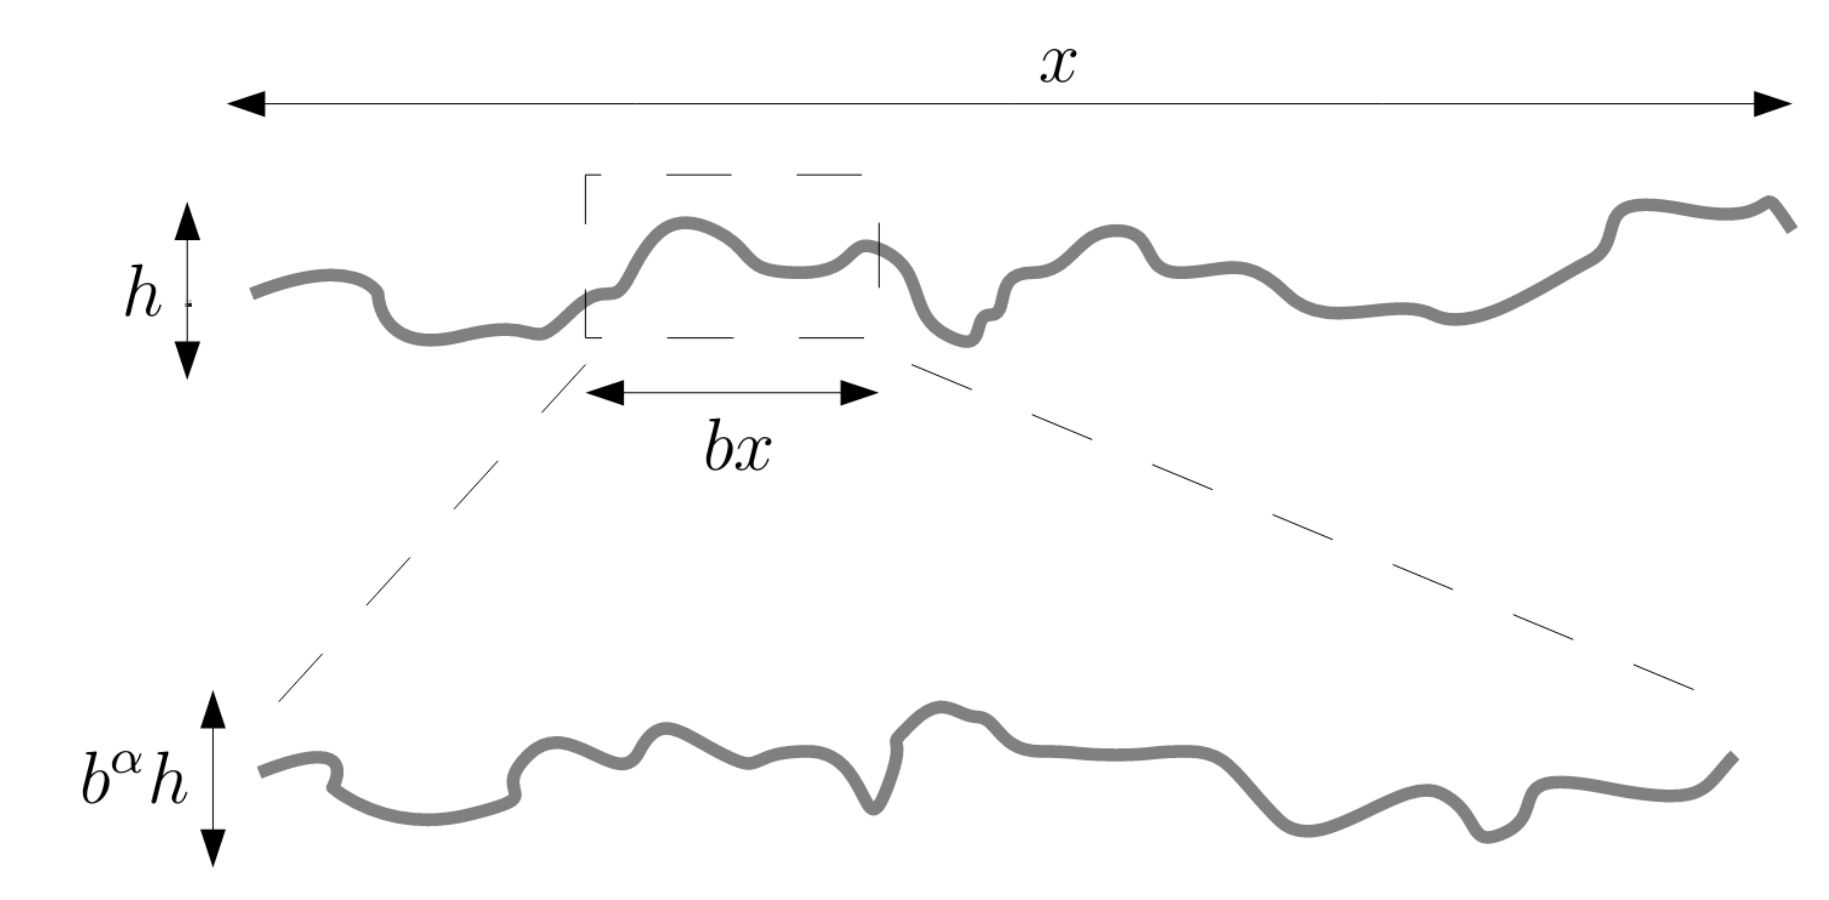
\includegraphics[width=\imsize]{self_aff.png}
    \caption[Auto-afinidad estadística.]{Auto-afinidad estadística: se muestra cómo el perfil de la interfaz permanece relativamente invariante ante una transformación anisotrópica.}
    \label{fig:self_aff}
\end{figure}

Por último, cuando la longitud de correlación $\xi_{||}(t)$ alcanza el tamaño del sistema $L$, similar a lo que pasa con el ancho, el factor de estructura deja de evolucionar y el sistema queda completamente correlacionado, con $S(q,t \gg t_x)\propto q^{-(1+2\alpha)}$.



\begin{figure}[!b]
    \hspace*{-1cm}
    \begin{subfigure}{.55\textwidth}
      \centering
      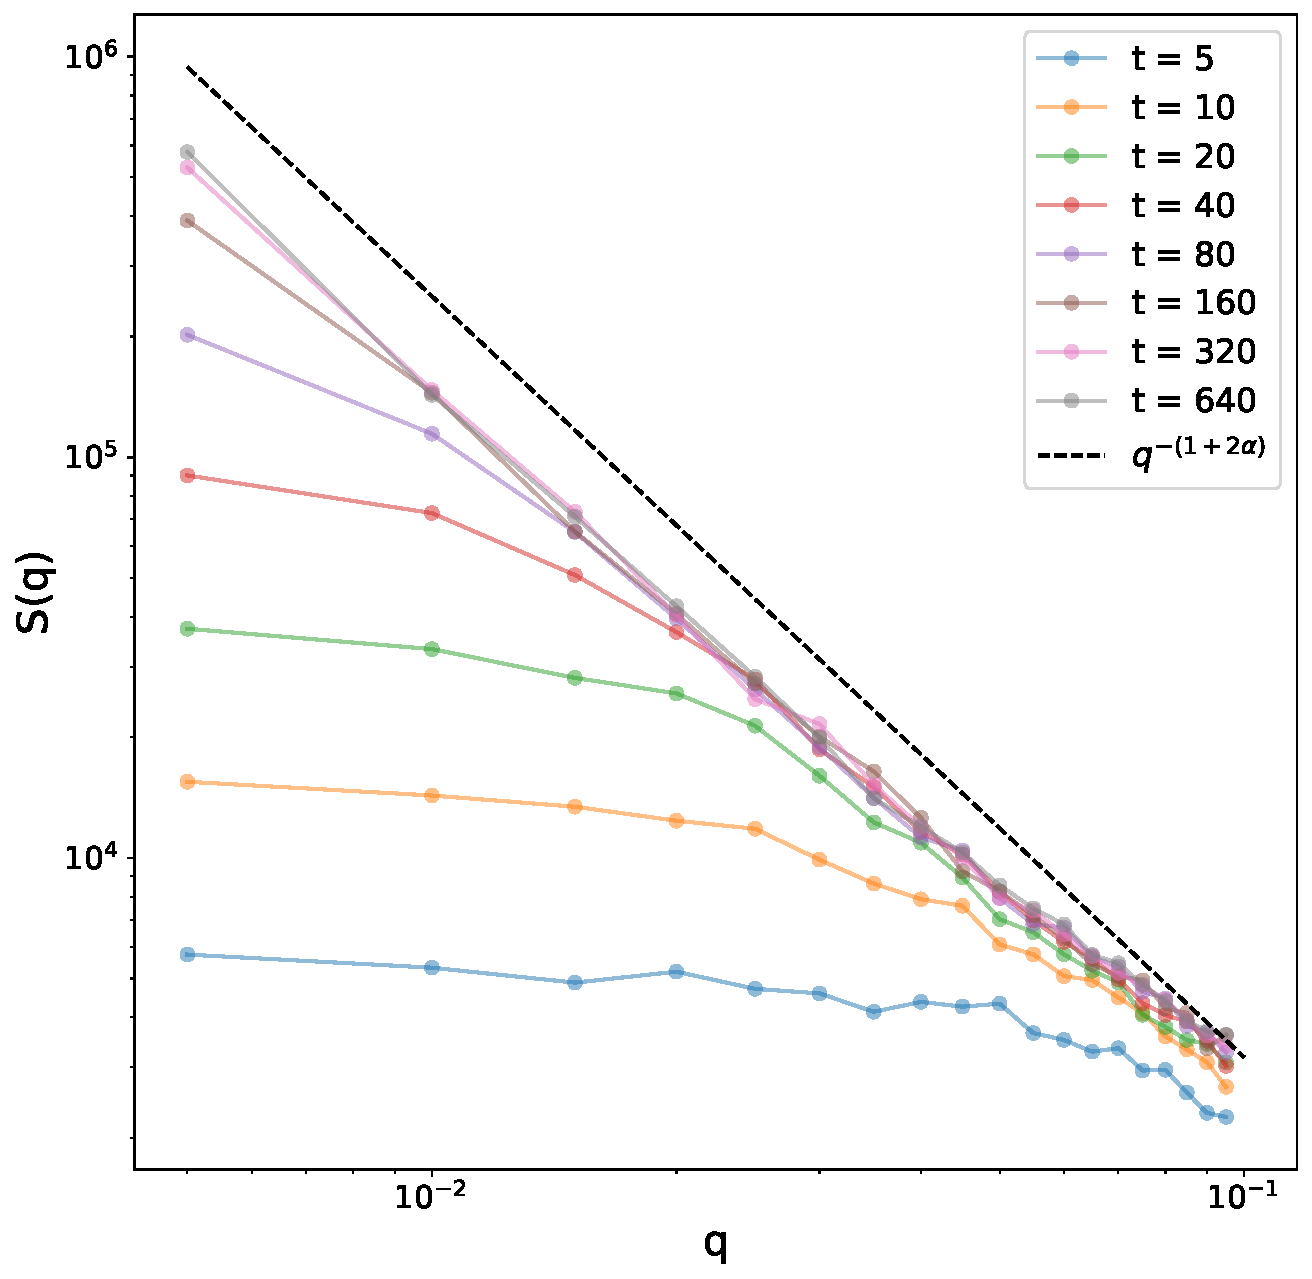
\includegraphics[width=\textwidth]{Sq.pdf}
      \caption{}
    \end{subfigure}
    \begin{subfigure}{.55\textwidth}
      \centering
      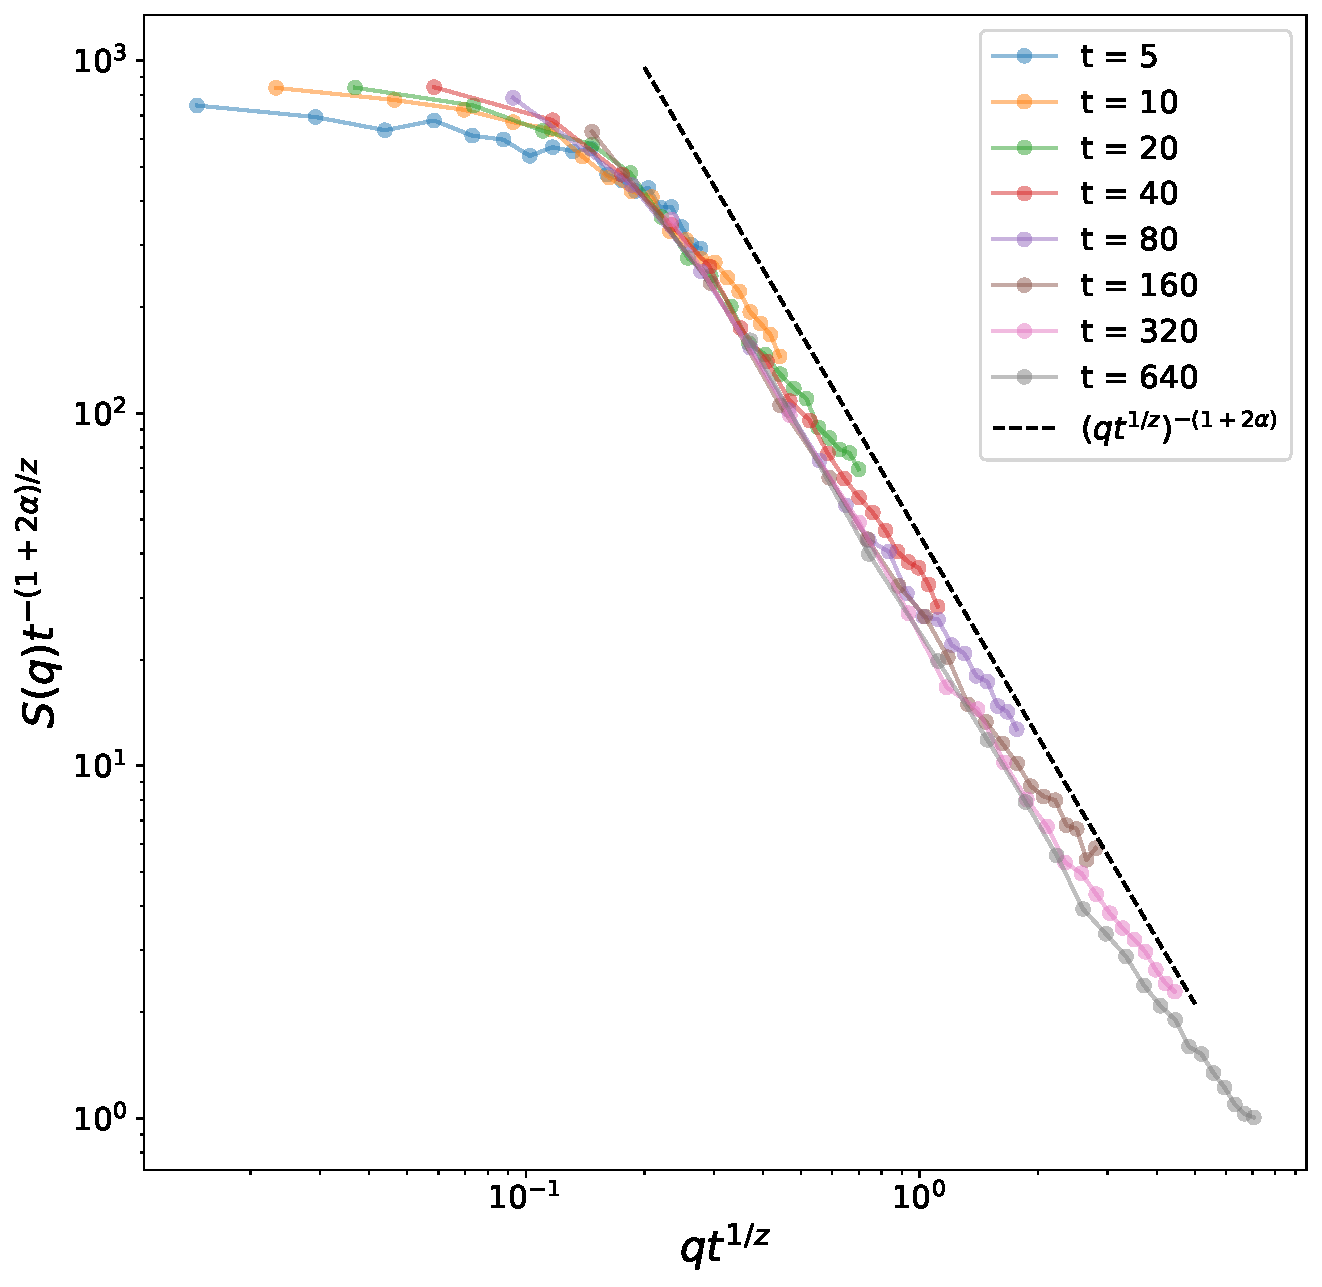
\includegraphics[width=\textwidth]{Sq_colapse.pdf}
      \caption{}
    \end{subfigure}
    \caption[Factor de estructura del modelo BD discreto.]{\textbf{(a)} Factor de estructura para el modelo BD discreto con $L=200$, $N=50000$ partículas y 500 realizaciones. \textbf{(b)} Colapso de las curvas que permite obtener los exponentes de rugosidad $\alpha$ y dinámico $z$.}
    \label{fig:structure_factor}
\end{figure}

En las figura \ref{fig:structure_factor}a se muestra el factor de estructura $S(q,t)$ para el modelo BD. Vemos cómo el mismo sigue la ley de potencias 
$S(q,t) \propto q^{-(1+2\alpha)}$ para $q \gg \xi_{||}(t)^{-1}$, mientras que para $q \ll \xi_{||}(t)^{-1}$ se comporta como $S(q,t) \propto t^{(1+2\alpha)/z}$, correspondiente a los \textit{plateaus}. De manera similar que con el ancho es posible escalear el factor de estructura para hacer que estas curvas colapsen en una sola, tal como se muestra en la figura \ref{fig:structure_factor}b. 

El factor de estructura ha mostrado ser más confiable a la hora de estimar el exponente de rugosidad $\alpha$ que a través del ancho de la interfaz, u otros observables
en el espacio real \cite{Bustingorry}, fundamentalmente porque regiones de escaleo diferentes aparecen claramente separadas en el espacio recíproco.




\sect{Universalidad: Poisson, KPZ y EW}{univ}


En la sección anterior se vio cómo el crecimiento de una interfaz puede ser caracterizado por un par de exponentes, por ejemplo $(\alpha,z)$. Estos exponentes 
definen lo que se conoce como la clase de \textit{universalidad} de la interfaz. Se dice universalidad dado que resulta que una gran diversidad de modelos que describen el crecimiento de una interfaz obedecen fundamentalmente las mismas relaciones de escala, independiente de los detalles del modelo.

Las tres clases de universalidad más conocidas son: Poisson, Edwards-Wilkinson (EW) y Kardar-Parisi-Zhang (KPZ) \cite{Family_1986,PhysRevLett.56.889}. En la primera, 
la altura de la interfaz en cada punto es independiente de la altura de los demás. En la segunda, las fluctuaciones son moderadas por términos difusivo que tienden a 
suavizar la interfaz. En la última, puntos cercanos de la interfaz se ayudan mutuamente para crecer, resultando en un efecto de amplificación no lineal de las fluctuaciones que compite con un término difusivo. Esta última descripción debiera recordarle el modelo BD, en donde los puntos alocados en cierta vecindad se ayudan mutuamente a crecer. En efecto, el modelo BD pertenece a la clase de universalidad KPZ en una dimensión.

Para estudiar las diferentes universalidades que pueden encontrarse, lo que se hace es proponer o bien derivar una ecuación diferencial estocástica que describa la evolución del campo de desplazamiento $h(x,t)$. Dicha ecuación para KPZ fue propuesta precisamente por Kardar, Parisi y Zhang \cite{PhysRevLett.56.889} y es la siguiente
\begin{equation}
    \frac{\partial h}{\partial t} = \nu \nabla^2h + \frac{\lambda}{2} \left(\nabla h\right)^2 + F + \eta(\mathbf{x},t), \quad \text{[KPZ]}
    \label{KPZ}
\end{equation}
donde el primer término de la derecha describe una relajación de la interfaz ejercida por una tensión superficial $\nu$ (o difusión si vemos a $h$ como una concentración), el término no lineal $\left(\nabla h\right)^2$ promueve el crecimiento de la interfaz en la dirección normal local de la misma, permitiendo así el crecimiento lateral. $F$ es una constante que podría ser el valor medio de la cantidad de partículas por unidad de tiempo que llega a la interfaz, es decir, $F=v_0 \simeq \partial_t h_m$. Mientras que el último término es un ruido que satisface
\begin{equation}
    \overline{\eta(\mathbf{x},t)} = 0, \quad \overline{\eta(\mathbf{x},t)\eta(\mathbf{x'},t')} = 2\kappa\delta^d(\mathbf{x}-\mathbf{x'})\delta(t-t'),
\end{equation}
donde $\overline{\cdots}$ denota promedio sobre realizaciones de ruido. La ecuación no lineal \ref{KPZ} puede resolverse de manera exacta en una dimensión $d=1$, lo que permite obtener los siguientes exponentes de escaleo\footnote{Los exponentes con d>1, no pueden determinarse analíticamente, sin embargo, se han obtenido numéricamente y pueden encontrarse reportados \cite{barabasi}.}
\begin{equation}
    \alpha = \frac{1}{2}, \quad z = \frac{3}{2} \quad \text{y} \quad \beta = \frac{1}{3}.
\end{equation}

El modelo BD es un modelo simple que ayuda a entender a nivel físico a qué se deben las características de la interfaz. Sin embargo, lo interesante es que 
es posible encontrar modelos más complejos que también pertenecen a esta clase de universalidad, más aún, resultados experimentales de fenómenos complejos muestran 
la dinámica de KPZ \cite{PhysRevE.96.013107,PhysRevE.74.041116}.

En las figuras \ref{fig:KPZ}a y \ref{fig:KPZ}b puede observar una representación gráfica del efecto que tienen sobre $h(x,t)$ el término difusivo o elástico $\nabla^2h$ y el término no lineal $\left(\nabla h\right)^2$ respectivamente, que aparecen en la ecuación \ref{KPZ}. 

De momento hemos hablado solo de KPZ, pero ¿qué queda para decir de las universalidades de EW y Poisson? Afortunadamente, KPZ es el más complejo de los tres dado que es no lineal, en lo que respecta a EW, la ecuación que describe su evolución es simplemente \ref{KPZ} pero con $\lambda=0$, es decir,
\begin{equation}
    \frac{\partial h}{\partial t} = \nu \nabla^2h + F + \eta(\mathbf{x},t). \quad \text{[EW]}
    \label{EW}
\end{equation}
que puede resolverse en cualquier dimensión obteniendo los exponentes de escaleo,
\begin{equation}
    \alpha = \frac{2-d}{2}, \quad z = 2 \quad \text{y} \quad \beta = \frac{2-d}{4}.
\end{equation}
Nótese que si $d>2$ entonces $\alpha<0$, lo que significa que la interfaz se contrae, se hace plana, cualquier perturbación que genere un ancho no nulo es suprimida por la tensión superficial.

\begin{figure}[!t]
    \hspace*{-1cm}
    \begin{subfigure}{.55\textwidth}
      \centering
      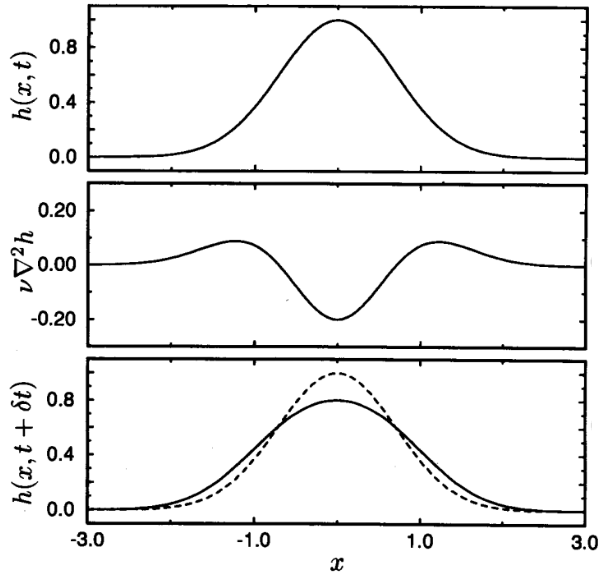
\includegraphics[width=\textwidth]{diffusive_term.png}
      \caption{}
    \end{subfigure}
    \begin{subfigure}{.55\textwidth}
      \centering
      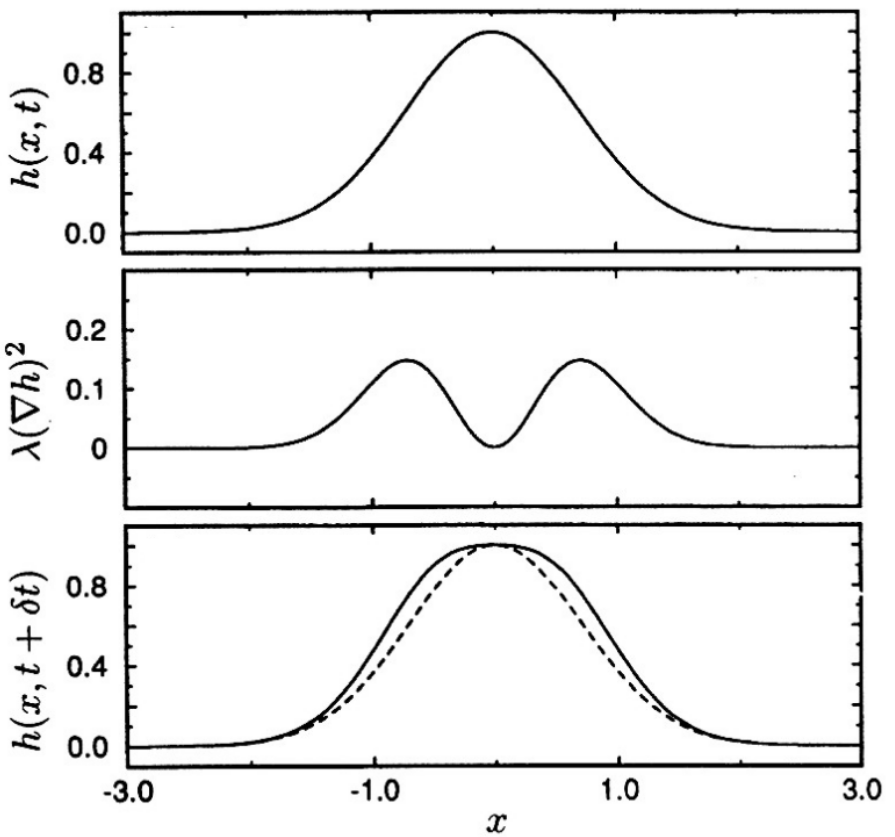
\includegraphics[width=\textwidth]{non_linear_term.png}
      \caption{}
    \end{subfigure}
    \caption[Término difusivo y no lineal de la ecuación de KPZ.]{Efecto sobre la interfaz $h(x,t)$ de \textbf{(a)} el término difusivo y \textbf{(b)} el término no lineal. Figuras extraídas de Ref. \cite{barabasi}.}
    \label{fig:KPZ}
\end{figure}

Por otro lado, un proceso de Poisson es, como podría esperar, uno en donde la interfaz crece de manera completamente aleatoria, la ecuación correspondiente es la siguiente,

\begin{equation}
    \frac{\partial h}{\partial t} = F + \eta(\mathbf{x},t). \quad \text{[Poisson]}
    \label{Poisson}
\end{equation}  
En este caso, únicamente tenemos un exponente, el exponente de crecimiento
\begin{equation}
    \beta = \frac{1}{2}, \quad \text{[Poisson]}
\end{equation}
dado que no hay un fenómeno de saturación para el ancho de la interfaz en un sistema finito, el ancho crece indeterminadamente, debido a la ausencia de correlación.

Ejemplos de modelo comunes que responden a Poisson y EW, son el crecimiento aleatorio y el crecimiento aleatorio con difusión, respectivamente. El primero es lo que se imagina, se crece la interfaz de manera aleatoria, las partículas caen aleatoriamente en un lugar y ahí quedan. La diferencia de este modelo con BD es que las partículas no pueden pegarse lateralmente a la interfaz. Por otro lado, en el crecimiento aleatorio con difusión, las partículas caen aleatoriamente y una vez que entran en contacto con la interfaz tienen permitido difundir cierta distancia hasta encontrar la altura mínima.

Un comentario final que será de importancia más adelante en el desarrollo de este trabajo, es sobre la velocidad de propagación de la interfaz para el caso de KPZ. Si uno integra espacialmente la ecuación \ref{KPZ}, promedia sobre desorden y define la velocidad media de propagación de la interfaz como
\begin{equation}
    v = \dot{h}_m(t) = \frac{d}{dt} \left(\frac{1}{L} \int_{0}^{L}d^d\mathbf{x} h(\mathbf{x},t) \right),
\end{equation}
resulta que la velocidad de propagación depende únicamente del término no lineal de \ref{KPZ}, 
\begin{equation}
    v = v_0 + \frac{\lambda}{2L} \int_0^L d^d\mathbf{x} \overline{\left(\nabla h\right)^2},
    \label{v_kpz}
\end{equation}
con $v_0=F$.











